\documentclass[11pt]{jsarticle}

\usepackage{SPR}

\headerSPR
\begin{document}
	\titleSPR{\number\year}{\number\month}{\number\day}{D2}{吉田 皓太郎}
%%%%%%%%%%%%%%%%%%%%%%%%%%%%%%%%%%%%%%
	\articleSPRabst
		\begin{itemize}
			\item 機械学習を用いたカップ形状の設計支援
			\item 着後形状予測のためのカップの変形解析
		\end{itemize}
		
		
	\articleSPRobj
		\begin{enumerate}
			\item 定性的な機能要求を満たせるようなカップ形状を設計できる
			\item 布の物性とカップのパターンがどのような結びつきを持っているかを調べることができる.
		\end{enumerate}
%%%%%%%%%%%%%%%%%%%%%%%%%%%%%%%%%%%%%%
% 1.前回からのノルマ
	\articleSPRitemsone
		%\begin{enumerate}
		%	\item A
		%\end{enumerate}
		
		\tableofcontents
		
		
%%%%%%%%%%%%%%%%%%%%%%%%%%%%%%%%%%%%%%
%\begin{itemize}
%	\item 新規手法について
%	\item ISFAアウトライン
%\end{itemize}
%%%%%%%%%%%%%%%%%%%%%%%%%%%%%%%%%%%%%%
% 2.具体的な成果
	\articleSPRitemstwo
	\renewcommand{\labelitemi}{$\blacktriangledown$}
%%%%%%%%%%%%%%%%%%%%%%%%%%%%%%%%%%%%%
	\section{研究進捗について}
		先週の研究成果等について報告いたします.
		\begin{itemize}
			\item 機械学習を用いたシステムの概要についての試行錯誤まとめ
			\item これからのTodo
		\end{itemize}
	\section{機械学習を用いたシステムの概要についての試行錯誤まとめ}
		システムの概要を以下に示す.
		\begin{figure}[H]
			\centering
			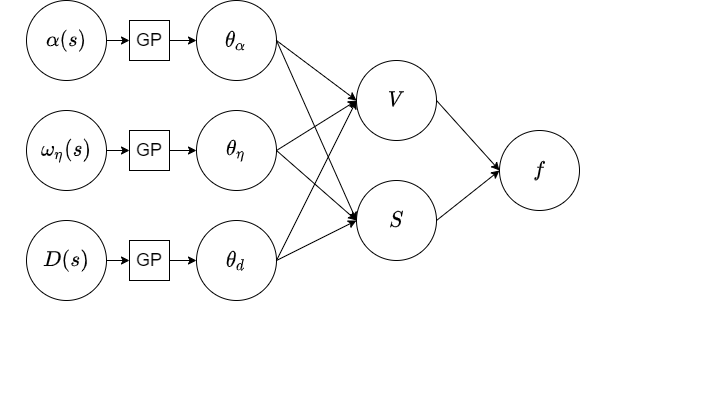
\includegraphics[scale=0.5]{./figure/systems.png}
			\caption{SYSTEM}
		\end{figure}
		\subsection{入力まわりの概要}
			ガウス・ボネの原理より,第一基本量,第二基本量によって可展面の情報は一意に決定される.これらの基本量は次式に示す形によって表されている.したがって,この可展面情報を一意に決定する関数群$ \alpha $,$ \omega_{\eta} , \omega_{\xi}$,$ D $を機械学習によって学習することができればよい.(厳密には$ D $は式中には出てこないが,$ t $の定義域が$ [0,D(s)] $であることから,特徴的であるとしている)
			\begin{eqnarray}
			E &=& (\alpha'+\lambda)^2 t^2 -2\cos \alpha(\alpha'+\lambda) t + 1,\\
			F &=& -\sin \alpha,\\
			G &=& 1,
			\end{eqnarray}
			
			\begin{eqnarray}
			L &=& -\omega_{\xi}+t\{\lambda(-\omega_{\xi}\cos \alpha + \omega_{\zeta}\sin \alpha)+\omega_{\zeta}'\cos \alpha + \omega_{\xi}'\sin \alpha \},  \\
			M &=& \omega_{\xi}\sin \alpha + \omega_{\zeta} \cos \alpha,  \\
			N &=& 0. 
			\end{eqnarray}
			また,先週にも述べたように,$  \omega_{\eta} , \omega_{\xi} $とワイヤーの空間曲率$ \kappa (s) $の間には,以下の関係が存在すること,また,データにおける前提としてワイヤーデータはすべて同じものを使っているということから,$ \omega_{\xi} $は$ \omega_{\eta} $に関して従属的に決定できる.
			\begin{equation}\label{eq:kappaeq}
			\omega_{\eta}^2 + \omega_{\xi}^2 = \kappa^2
			\end{equation}
			このことから,$ \omega_{\xi} $は特徴量から除外でき,可展面を決定するのは関数群$ \alpha $,$ \omega_{\eta} $,$ D $の3つの関数である.
		\subsection{入力をなぜGPで表現したか}
			タイトルの件について,おそらく研究会の説明等では不足であると考え,追記します.
			
			この表現の目的はある関数$ f(x) $の特徴を記述するパラメータを入力パラメータとしたいと考えたところから出発します.最も単純で馴染みの深い方法としては,下記のように$ f(x) $を基底関数$ \bd{\phi} = \{ \phi_i(x) \} $の重み付き線形和によって表現する方法です.
			\begin{equation}\label{eq:LinearEq}
				f(x) = \sum_{i=0}^{N} w_i \phi_i(x)  = \bd{\phi} \bd{w}
			\end{equation}
			入力のデータセット$ \bd{x} = \{x_i\} $出力データセット$ \bd{\hat{f}} = \{\hat{f}_i\}$が与えられている場合,$ \bd{w} $は次のような二乗誤差を最小化することで得られる.
			\begin{equation}\label{eq:ErrorToMinimize}
				E =  \sum_{i=0}^{N} (\hat{f}_i - \sum_{j=0}^{N} w_j \phi_j(x_i))^2
			\end{equation}
			しかしこの場合,$ \dim(\bd{w}) $をどの程度であればよいのかは関数毎に設定が必要である点や,パラメータの次元が増加してしまう,などの問題があります.
			
			ガウス過程では,この$ \bd{w} $があるガウス分布$ \mathcal{N}(\bd{0},\lambda^2 \bd{I}) $から生成されたものと仮定します.この場合,出力の$ f $もまたガウス分布に従います.平均と分散はそれぞれ次式のように計算されます.
			\begin{equation}\label{eq:Avg}
				\bd{m} = \mathbb{E}(f(x)) = \bd{\phi} \cdot \mathbb{E}( \bd{w}) = \bd{0}
			\end{equation}
			\begin{equation}\label{eq:Var}
				\bd{\sigma} = \mathbb{E}(\bd{f} - \bd{m})^2 = \lambda^2  \bd{\Phi}  \bd{\Phi}^{\mathrm{T}}
			\end{equation}
			ただし,$ \bd{\Phi} =\{\phi_j(x_i) \}$とおいております.これを$ \bd{K} = \lambda^2  \bd{\Phi}  \bd{\Phi}^{\mathrm{T}} $とおくと$ \bd{K} $は$ f $の共分散行列となり,$ f $はガウス分布$ \mathcal{N}(\bd{0},\bd{K}) $に従い,$ \bd{K} $の各成分は$ k_{i,j} = \bd{\phi}(x_i) \bd{\phi}^{\mathrm{T}}(x_j) $となります.この時$ f $のガウス分布を求めるためには,$ \bd{\phi} $を設計するのではなく,$ k_{i,j} $を直接設計すればよいことが分かります.このようなテクニックはカーネルトリックと呼ばれ,$ k_{i,j} $をカーネル関数と呼びます.
			
			重要な点は2点で,一つは$ \dim(\bd{\phi}) $の次元が無限としても,$ k_{i,j} $が有限の値を持つようであれば構わないという点で,もう一つの点は,ガウス過程の出発が基底関数の線形和で表すというRitz法と考え方が等価である点です.
			
			したがって,カーネル関数を決定するいくつかのパラメータを適切に設定さえすれば,$ f $をガウス分布によって表現でき,これにより,パラメータの次元増加を避けることができると考えられます.カーネル関数のパラメータを求める際には,対数尤度最適の考え方が用いられ,確率分布の対数をとった関数が最大化するようにパラメータを最適化します.
			\begin{equation}\label{eq:Suudo}
			\log(p) = -\log|\bd{K}_{\theta}| - \bd{y}^T \bd{K}_{\theta}^{-1} \bd{y}+C
			\end{equation}
			
		\subsection{試行錯誤の過程で変えた点など}
			まず,これまでの試行によって得られていた課題について,次のような課題がありました.
			\begin{itemize}
				\item 外れ値が大きい
				\item 計算にこんなパラメータいる?
			\end{itemize}
			\begin{itemize}
				\item 与えられた3つの関数のデータセット$ (s_i,f(s_i)) $が与えられ,GPを用いてハイパーパラメータを抽出する時,これまでカーネル関数を次式のようにしていました.
				\begin{equation}\label{eq:RBFLinear}
				k(x_i,x_j) = \theta_1 \exp \left( -\frac{(x_i-x_j)^2}{\theta_2} \right) + \theta_3 x_i x_j
				\end{equation}
				さらに,今回はPythonのガウス過程ライブラリGPyを用いて行っているため,デフォルトで誤差の分散がパラメータに追加されており,合計のパラメータは$ 4*3=12 $個となっていました.しかし,値を精査すると,線形項および分散パラメータは小さくあまり意味をなしていないことが分かったため,これを取り除き,結果として$ 2*3=6 $個のパラメータで計算を行いました.最も分散パラメータは,元々ばらつきを持つデータ用にあるものなので,意味をなさないのは当然ですが・・・.
				\item 評価関数を
				\begin{equation}\label{eq:EvalFunc}
				f(V,S) = \phi_1 \frac{\Delta V}{V_b} \exp \left(-\phi_2 \left(\frac{\Delta S}{S_b}\right)^2 \right)
				\end{equation}
				としていましたが,これだと外れ値が多く出てしまい,既存のデータセットではちょっと評価がしづらかったです.そこで,次のような思考の下,評価関数を変えました.
				
				ブラジャーカップにおける「上げる」機能に着目します.この「上げる」機能は,カップ曲面の面積に対し,どれだけ体積があるかを求めることで得ることができる,つまりある意味での,広義の「高さ」によって決定できると考え,評価関数を次のように決定しました.
				\begin{equation}\label{eq:EvalFunc2}
				f(V,S) = \phi_1 \frac{V_{cup}}{S_{cup}}
				\end{equation}
			\end{itemize}
		\subsection{結果}
			今回は$ \phi_1 $のパラメータを$ 30 $に設定し,カーネル関数を次式のように設定しました.
			\begin{equation}\label{eq:KernelForExperiment}
				k(\bd{x},\bd{y}) = \sigma^2 \bigg( 1 + \frac{1}{2} \sum_{p=1}^{N} \frac{(x_i-y_i)^2}{\theta_{p,r}^2} \bigg)^{- \alpha} + \sum_{p=1}^{N} \theta_{p,l} x_p y_p
			\end{equation}
			また,現在,学習データが1093個程度あり,これを
			\begin{itemize}
				\item 学習用データ 900個
				\item 検証用データ 193個
			\end{itemize}
			に分けて,結果を示します.
			\bfig[H]
			\centering
			\bmini{0.5\textwidth}
			\centering
			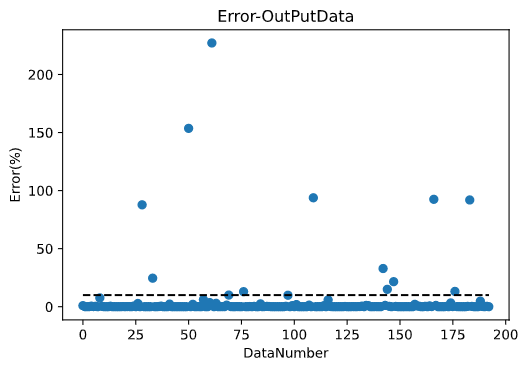
\includegraphics[scale=0.4]{./figure/ErrorForOutputDataGraph.png}
			\caption{Error of Output Data}
			\emini
			\bmini{0.5\textwidth}
			\centering
			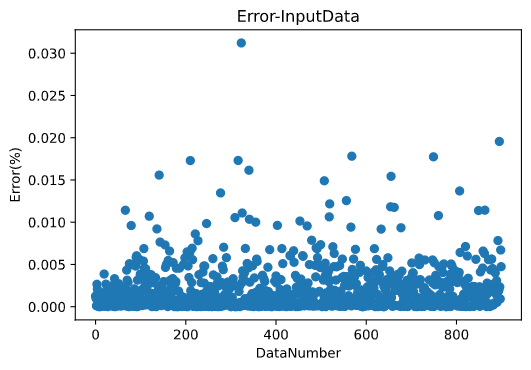
\includegraphics[scale=0.4]{./figure/ErrorForInputDataGraph.png}
			\caption{Error of Input Data}
			\emini
			\efig
			
			\bfig[H]
			\centering
			\bmini{0.5\textwidth}
			\centering
			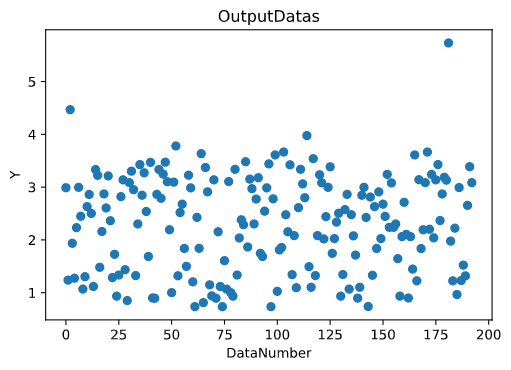
\includegraphics[scale=0.4]{./figure/OutputData.png}
			\caption{Output Data}
			\emini
			\bmini{0.5\textwidth}
			\centering
			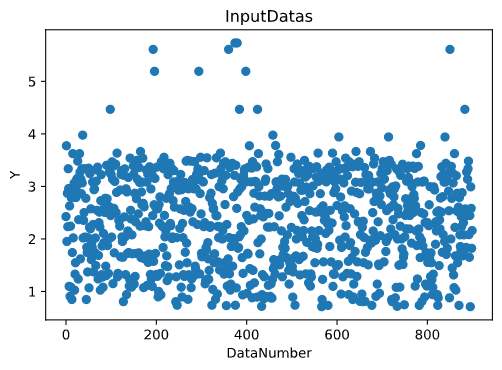
\includegraphics[scale=0.4]{./figure/InputData.png}
			\caption{Input Data}
			\emini
			\efig
			
			\bfig[H]
			\centering
			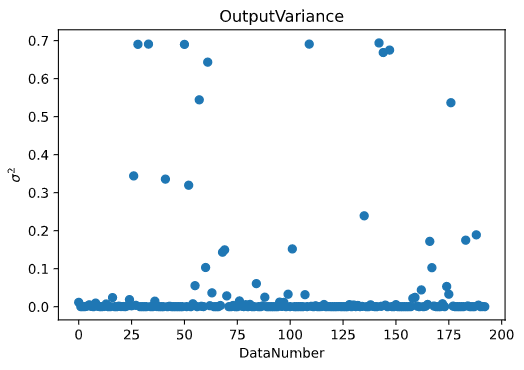
\includegraphics[scale=0.4]{./figure/OutputVariance.png}
			\caption{Variance of Output Data}
			\efig
			
			ただし,誤差の単位は($ \% $)で,縦軸が10のところでは横線を引いており,誤差が$ 10\% $以上のものがいくつあるかを視覚化しております.なお,二乗平均平方根誤差(RMSE)は0.24641777673600893で,決定係数は0.9217558814177508でした.決定係数から行くと,このモデルは当てはまりがよいことが分かります.
			
			外れ値の部分に関してはどうしようもなく,誤差が大きくでてしまいますが,全体としてよく近似できていると考えることができるのでは,と結論づけます.(この部分に関してはもしかしたらデータ自体がおかしい可能性も否定できないので,要注意です・・・)
			
			また,ガウス過程のよいところとして,解の予測度を同時に出力できる部分で,実際に事後分散が大きいところと,誤差の大きいところの傾向が似ていることが見て取れるかと思います.(もしかしたらグラフでは読み取れないかもしれませんが,実際にデータを見比べると,ピークの出る位置が似ております)
			
			つまり,解を推測した段階で,誤差を調べずともその推測精度みたいなものが分かります.
				
		\subsection{これからのTodo}
			\begin{itemize}
				\item 評価関数の正当性みたいなものは再検討してもいい.
				\item データを作り直し,二枚接ぎカップ全体で学習用データを作りたい.
				\item 機能の値にしたがって解が出てくるような手法,深層学習の適用
				\item ISIGHT上でAbaqusを実行できるか,最適化の実行(適当な関数を設定すればいいので)
				\item objファイル$\rightarrow$igsファイルへ変換する方法教えてください.(マクロ化して実行するため)
			\end{itemize}
			
	\newpage
\vspace{10cm}
%%%%%%%%%%%%%%%%%%%%%%%%%%%%%%%%%%%%%%
% 3.達成できなかったこととその問題点
	%\articleSPRthree
	
%%%%%%%%%%%%%%%%%%%%%%%%%%%%%%%%%%%%%%

\vspace{14cm}
%%%%%%%%%%%%%%%%%%%%%%%%%%%%%%%%%%%%%%
	\articleSPRfour
	\articleSPRfive
\end{document}
